%!TEX root = ../MainBody.tex

% 第一章
% ═══════════════════════════════════════════════════════════════════
% 写作思路（全章概要）：
%   绪论作为论文入口，需完成三个任务：
%   (1) 说明红外仿真的重要性和现有方法局限 → 建立研究动机
%   (2) 综述相关领域研究进展 → 定位本文贡献
%   (3) 概括研究方案和论文结构 → 为后续章节铺路
%
%   逻辑链：应用需求 → 方法局限 → 技术机会 → 本文方案
% ═══════════════════════════════════════════════════════════════════
\chapter{绪论}% 使用\cite{}命令引用数据库中文献

\section{研究背景及意义}
%% 写作思路（本节）：
%%   第一层：红外仿真的应用价值——军事（目标识别/制导）、工业（热管理/缺陷检测）、
%%           建筑（热桥检测）、医学（体温监测）
%%   第二层：红外仿真的核心挑战——与可见光渲染相比，红外过程涉及辐射+传导+对流
%%           多物理耦合，计算量远大于单一物理过程
%%   第三层：传统方法的局限——有限元/有限体积法需离散全域网格，耦合求解要迭代外循环；
%%           解耦方法（各物理分别求解再耦合）精度低、物理不自洽
%%   第四层：蒙特卡洛路径追踪方法的优势——统一路径空间、无网格、天然耦合
%%           但计算量大（每像素需数千条路径），效率是核心瓶颈
%%   第五层：GPU 加速的技术机会——RT Core 硬件光追 + 大规模并行
%%           → 引出本文"混合架构耦合热输运"的研究必要性
%%
%% [篇幅需求] 约800字。
%% [引用需求] 红外仿真综述/应用：需补充红外仿真领域的综述性文献
%%   - 填充下方 \cite{} 中的空引用，建议查找红外仿真/红外场景生成领域的综述文章
%%   - 可考虑引用 WangTingJiYuMonteCarloFangFaDeWuHongWaiChuanShuFangZhenJiFenXi2018
%%   - 可考虑引用 YuLiangYuJiYuLuJingZhuiZongDeSanWeiHongWaiChangJingFangZhenSuanFaJiShiXian2020
%% [引用需求] 有限元/有限体积法在热仿真中的应用：需补充传统数值方法的文献
%% [引用需求] GPU 计算/RT Core 相关综述
%%
红外仿真在军事、工业、医疗等领域具有重要应用价值，是红外科学中获取红外辐射特性、分析红外系统性能、设计红外设备的重要工具\cite{upadhyayComprehensiveSurveySynthetic2025,LuQiHongWaiChangJingFangZhenFangFaJiFaZhanXianZhuangYanJiuZongShu2024,WangXiaHongWaiChangJingFangZhenJiShuFaZhanZongShu2015}。在军事领域，红外仿真用于生成目标与背景的合成红外图像，支撑导弹红外导引头的半实物仿真测试、战场目标红外特征预测与对抗策略评估\cite{upadhyayComprehensiveSurveySynthetic2025}；在航天领域，航天器在轨热控设计依赖对太阳辐射、地球红外辐射与深空冷背景联合作用下的热平衡仿真，以验证星载仪器在极端温度环境下的工作可靠性\cite{modestRadiativeHeatTransfer2013}。然而，与可见光渲染仅涉及辐射传输不同，红外成像本质上是一个多物理耦合问题：辐射、传导、对流三种热输运机制通过固-流界面处的能量守恒方程相互关联、无法独立求解。这一耦合特性既决定了红外仿真的工程价值——能够预测复杂真实场景下的温度场与辐射分布，也构成了其计算建模的根本难点，是后续各类方法演进所共同面对的核心问题。

围绕这一难点，已有研究形成两条主线。一是以有限元法、有限体积法为代表的确定性数值方法，将求解域离散为网格单元后分别建模各物理过程，再通过外循环迭代在界面处交换边界数据；其收敛精度与效率受迭代策略与网格质量的双重制约，在强耦合场景下尤为困难\cite{modestRadiativeHeatTransfer2013}。二是借鉴计算机图形学渲染管线的方法，将辐射过程独立求解后再与传导、对流结果耦合，效率较高但本质上仍属解耦近似，物理自洽性不足。由于上述两类方法的共同短板均源自"解耦"假设，近年来基于路径追踪的蒙特卡洛方法在统一的随机路径空间中同时采样三种热输运过程\cite{batiCouplingConductionConvection2023}，从方法论层面回避了解耦近似，确立了物理自洽的耦合热输运求解框架。然而该框架的工程化落地仍面临突出瓶颈：每条耦合路径内含数十至上百次密集的几何查询（光线求交与最近面投影），且递归求解结构导致路径间无法并行，使其计算效率严重受限于几何查询吞吐，传统 CPU 光追库已难以胜任。在此前提下，NVIDIA RTX 系列 GPU 提供的 RT Core 硬件加速光线追踪能力日趋成熟，为突破上述瓶颈提供了硬件基础——这正是本文的切入点：在保留蒙特卡洛耦合热输运物理自洽性的同时，将递归求解重构为可并行的 Wavefront 调度，并把批量几何查询卸载至 GPU 硬件光追后端，从而在物理一致性的前提下显著提升仿真效率。下节将围绕这一演进脉络系统综述国内外研究现状，定位本文在其中的位置。


\section{国内外研究现状}
%% 写作思路（本节）：
%%   文献综述需覆盖四个维度，与第二章理论基础形成"广度 vs 深度"的互补：
%%   - 本节侧重学术脉络、发展趋势、不同方法的优劣比较
%%   - 第二章侧重本文实际使用的理论和技术的详细阐述
%%   注意避免与第二章内容重复，此处点到为止、重在评述。
%% [篇幅需求] 约3000-4000字。

红外仿真方法的研究进展体现为一条由技术瓶颈驱动的演进链\cite{upadhyayComprehensiveSurveySynthetic2025,LuQiHongWaiChangJingFangZhenFangFaJiFaZhanXianZhuangYanJiuZongShu2024,WangXiaHongWaiChangJingFangZhenJiShuFaZhanZongShu2015}：从早期经验与半经验建模，到基于第一性原理的数值仿真，再到引入图形学渲染技术的辐射仿真，进而发展出在单一路径空间统一求解辐射、传导、对流三种热输运机制的蒙特卡洛路径追踪框架；GPU并行光追硬件的迅速发展，则为突破该框架当前的计算效率瓶颈提供了技术基础。每一阶段的出现，均是对前一阶段遗留瓶颈的针对性回应，以下各节依次阐述。

\subsection{经验与半经验方法}

最早的红外仿真系统出现于20世纪80年代，以经验和半经验建模方法为主。这类工作通过对目标和背景建立简化热模型，利用有限的测量数据标定参数，生成合成红外图像，较早的工作如\cite{jacobsSimulationThermalBehaviour1980,ben-yosefSimulationIRImages1983,kornfeldComputerGenerationInfrared1985}。这类方法计算效率高，但物理精度有限，泛化能力不足，主要用于训练模拟器等对精度要求不高的场景\cite{bieselRealtimeSimulatedForward1987}。

大气传输是红外成像链路的重要组成部分。LOWTRAN\cite{kneizysAtmosphericTransmittanceRadiance1978}和MODTRAN\cite{MODTRANModerateResolution1987,berkMODTRAN6MajorUpgrade2014}等大气传输代码基于分子吸收谱线数据库，通过半经验积分方法计算大气透过率与辐射率，至今仍是红外工程中大气效应建模的标准工具。

随着建模精度需求的提升，研究者将简化热模型逐步拓展至涵盖昼夜热循环\cite{curtisDiurnalSeasonalVariation1990}、地形-目标热交互\cite{gondaExplanationVehicleterrainInteraction2003}以及传感器辐射链路各环节综合分析\cite{nandhakumarIntegratedAnalysisThermal1988}等复杂效应。进入21世纪，多光谱与高光谱热成像仿真\cite{kwanSimulationHyperspectralThermal2008}和多尺度场景辐亮度建模\cite{naraniyaSceneSimulationModeling2021}研究相继出现，进一步拓展了半经验框架在复杂战场环境下的工程应用边界\cite{haynesAccurateSceneModeling2003}。

在材质建模方面，红外波段的双向反射分布函数（BRDF）建模是提升仿真保真度的关键\cite{priestPolarimetricMicrofacetScattering2002}。半经验方法通过参数化材质模型，辅以物理约束，在计算效率与仿真精度之间取得折衷\cite{balfourSemiempiricalModelbasedApproach1997,schottIncorporationTextureMultispectral1995}。以 MuSES\cite{johnsonMuSESNewHeat1998}和 DIRSIG\cite{meyersModelingPolarimetricImaging2002}为代表的全链路集成仿真系统，综合了热辐射分析与大气传输模型，实现了目标-背景-大气-传感器的完整红外成像链路仿真，形成了该方向的系统方法论\cite{gondaComprehensiveMethodologyThermal1989}。然而，经验与半经验方法的精度高度依赖模型参数的获取质量，对多材质、复杂几何和强多物理耦合场景的外推能力有根本局限。

\subsection{基于数值求解的物理仿真方法}

为突破经验方法的精度瓶颈，基于第一性原理的物理仿真思路逐渐成为主流。\citeauthor{shefferComputerGeneratedIR1988}最早将物理建模方法引入红外图像生成，以辐射能量守恒为基础构建目标的热特征物理模型\cite{shefferComputerGeneratedIR1988}。

在传热仿真方面，有限元法（FEM）和有限体积法（FVM）是求解传导和对流问题的经典手段：将求解域离散为网格单元，对偏微分方程（傅里叶定律、Navier-Stokes 方程）施加局部守恒约束，迭代求得温度场\cite{patankarNumericalHeatTransfer1980,bergmanFundamentalsHeatMass2011}。辐射传输方程的数值求解则通常采用离散坐标法（DOM/S$_N$ 方法），将连续的角度空间离散为有限方向集，从而将积分-微分方程转化为代数线性方程组\cite{fivelandDiscreteOrdinatesSolutions1984,modestRadiativeHeatTransfer2013}。

\citeauthor{kottlerPhysicallybasedThermalSimulation2019}针对城市大规模航空红外热仿真需求，提出了"航空影像随机森林材质分类—四叉树约束三角化网格生成—三维有限体积法热仿真"四步流水线，在澳大利亚 Melville 城市实测数据集上耗时252秒完成了5个昼夜循环的温度场仿真，并通过定量对比验证了流水线的工程准确性\cite{kottlerPhysicallybasedThermalSimulation2019}。然而，上述确定性数值方法在处理辐射、传导、对流多物理耦合时，通常将三种过程分别建模，通过界面条件在外层迭代循环中交替求解。这种解耦策略在各物理过程弱耦合时效果良好，但在强耦合场景（如高温固体辐射与气体对流共存）中，界面热流的非线性高度敏感于局部温度，外层迭代收敛缓慢甚至不收敛\cite{modestRadiativeHeatTransfer2013,howellThermalRadiationHeat2021}。此外，FEM/DOM 的离散精度受网格分辨率制约，细节丰富的复杂目标场景（如战场车辆与背景地形的精细几何）所需网格规模极大，生成成本高昂且对几何质量高度敏感，构成实际工程应用的重要瓶颈。\cref{fig:fem_grid_example}展示了典型红外仿真对象的三角形网格——即便是单一目标，其几何复杂度也已要求大规模面片离散。从根本上看，基于网格的确定性数值方法将辐射视为网格单元间的热流交换，而非携带方向信息的光子输运，这使其难以自然融入光线追踪、重要性采样等计算机图形学的高效方法体系。

\begin{figure}[htbp]
  \centering
  \begin{subcaptiongroup}
  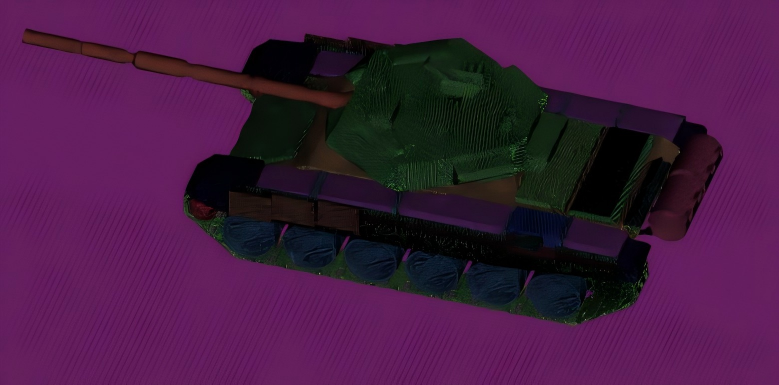
\includegraphics[width=0.46\textwidth]{Figures/FEM_Object_Grid_Example/Tank_Grid.png}
  \hfill
  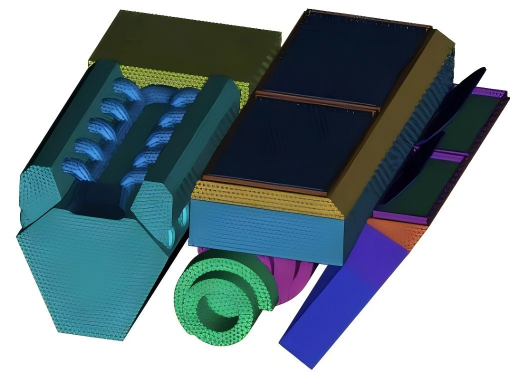
\includegraphics[width=0.46\textwidth]{Figures/FEM_Object_Grid_Example/Tank_Engine_Grid.png}
  \end{subcaptiongroup}
  \bicaption{红外仿真目标场景的三角形网格示例\cite{XuZhenDaoTanKeMuBiaoYuFuZaDiMianBeiJingOuHeReHongWaiTeZhengYanJiu2023}}{Example triangle meshes of infrared simulation target scenes~\cite{XuZhenDaoTanKeMuBiaoYuFuZaDiMianBeiJingOuHeReHongWaiTeZhengYanJiu2023}}
  \label{fig:fem_grid_example}

  \small
  坦克整车（左）与发动机舱部件（右）。
\end{figure}

\subsection{基于全局光照的辐射仿真方法}

1.2.2节的确定性数值方法将辐射视为网格单元间的热通量交换而非携带方向信息的光子输运，在处理复杂几何场景的多次反射与遮挡关系时受到根本制约，也难以融入光线追踪等计算机图形学方法体系。计算机图形学领域的全局光照技术——辐射度方法与光线追踪——为这一局限提供了解决思路；将其引入红外波段，可在不依赖角度离散的情况下高效处理几何复杂场景。\citeauthor{coiroGlobalIlluminationTechnique2013}较早在飞行器红外特征精确计算问题中将蒙特卡洛光线追踪全局光照模型集成至ONERA CRIRA仿真代码，采用Z缓冲器可见性判别、八叉树空间划分与重要性采样三重加速策略，实现了机身、进气道等部件间多重漫反射耦合的精确建模，证明了腔体部件的全局光照建模对辐亮度计算的影响可达$\pm$15\%\cite{coiroGlobalIlluminationTechnique2013}。

实时渲染需求推动了GPU加速红外仿真的快速发展。在辐射度精确渲染方向，\citeauthor{huangGPUbasedHighprecisionRealtime2014}通过有效平均值分解将谱耦合辐射方程转化为"原辐亮度$\times$有效平均因子"乘积形式，将多维参数预计算为三维GPU纹理查找表，实现了高精度实时辐射度渲染\cite{huangGPUbasedHighprecisionRealtime2014}；\citeauthor{wuRealtimeMidwavelengthInfrared2015}针对中波红外辐射仿真，提出了同时满足Helmholtz互易性与能量守恒约束的谱相关BRDF模型，构建了PRISSE集成仿真系统并通过实测光谱数据验证了其宽角度适用性\cite{wuRealtimeMidwavelengthInfrared2015}；\citeauthor{liRealtimeMultiresolutionRendering2018}针对超大规模地形背景，将遥感影像材质分类（$\kappa\approx0.9$）、简化能量平衡模型与15级多分辨率纹理金字塔结合，借助外存渲染技术实现了超过200~GB地形数据的无缝实时红外渲染\cite{liRealtimeMultiresolutionRendering2018}。

国内研究者在基于图形引擎的场景驱动方向进行了系统探索。\citeauthor{PanXuePingJiYuCreatorHeVegaDeHongWaiFeiXingShiJingFangZhen2007}利用Creator建模工具与Vega SensorVision传感器模块，结合预计算大气辐射传输查找表，构建了夜视飞行目标红外视景仿真系统\cite{PanXuePingJiYuCreatorHeVegaDeHongWaiFeiXingShiJingFangZhen2007}；\citeauthor{LinKaiJiYuOGREDeDongTaiHongWaiChangJingFangZhenYanJiu2010}在OGRE开源渲染引擎上整合"目标—背景—大气—成像系统"综合模型，在60~km$\times$60~km大场景下实现了82~fps实时双波段渲染，并以渲染合成器管线仿真了MTF、噪声和渐晕等成像效应\cite{LinKaiJiYuOGREDeDongTaiHongWaiChangJingFangZhenYanJiu2010}；\citeauthor{YangBoJiYuOSGDeHongWaiShiJingFangZhenYanJiu2017}在OSG引擎上提出了基于材质类别与相对高度的大规模地形动态分块调度方案，解决了空地导弹攻击场景下超大地形实时渲染的加载瓶颈\cite{YangBoJiYuOSGDeHongWaiShiJingFangZhenYanJiu2017}；\citeauthor{WangJunDiHaiMianHongWaiChangJingShengChengJiShuYanJiu2020}通过对实测光谱热特性数据的统计分析，系统化构建了地面车辆与海面舰船目标的全天候24小时红外场景生成系统\cite{WangJunDiHaiMianHongWaiChangJingShengChengJiShuYanJiu2020}；\citeauthor{LiWeiQingMianXiangShuZiLuanShengZhanChangDeHongWaiChangJingShiShiFangZhenFangFa2022}借助有限自动机对红外仿真计算流图进行并行化形式化分析，从理论上证明了多类原子并行结构的可行性，并构建了面向数字孪生战场样本生成的实时仿真系统\cite{LiWeiQingMianXiangShuZiLuanShengZhanChangDeHongWaiChangJingShiShiFangZhenFangFa2022}。

在与本文方法路线更为接近的高精度方向，\citeauthor{XuFeiFanJiYuOptiXBingXingGuangXianZhuiZongJiSuanDeHongWaiChengXiangFangZhenRuanJianYanZhi2022}将OptiX并行光线追踪与蒙特卡洛辐射传输相结合，引入Streaming RIS重要性采样策略与循环降噪自编码器，构建了支持中远红外双波段的高真实感仿真软件，验证了GPU硬件光追路线在红外成像仿真中的工程可行性\cite{XuFeiFanJiYuOptiXBingXingGuangXianZhuiZongJiSuanDeHongWaiChengXiangFangZhenRuanJianYanZhi2022}；\citeauthor{YuLiangYuJiYuLuJingZhuiZongDeSanWeiHongWaiChangJingFangZhenSuanFaJiShiXian2020}将蒙特卡洛路径追踪框架延伸至红外辐亮度积分与大气传输路径积分，通过OpenGL着色器实现GPU并行加速，是国内较早探索将路径追踪引入三维红外场景仿真的研究之一\cite{YuLiangYuJiYuLuJingZhuiZongDeSanWeiHongWaiChangJingFangZhenSuanFaJiShiXian2020}。

然而，上述基于全局光照的方法虽能有效处理辐射传输与光学遮挡，但无论渲染工具如何精进，热传导与热对流始终作为独立的预处理步骤通过温度场输入驱动辐射仿真，三种热输运机制从未在同一计算框架内统一建模。这种解耦从原理上限制了系统对动态热平衡、瞬态传热和材料内部热扩散的建模能力，也无法从路径空间角度对三种机制的耦合贡献进行统一采样与分析。

\subsection{基于路径追踪蒙特卡洛热输运仿真方法}
%% 写作思路：本节是文献综述的核心，直接支撑本文的方法论基础
%%   (1) 蒙特卡洛方法在热辐射中的早期应用
%%       - Howell (1964, 1969) 开创性工作 → \cite{howellMonteCarloSolution1964,howellApplicationMonteCarlo1969}
%%       - Kac (1947) 随机游走理论 → \cite{kacRandomWalkTheory1947}
%%   (2) 路径追踪在辐射传输中的发展
%%       - null-collision 方法 → \cite{galtierIntegralFormulationNullcollision2013}
%%       - Villefranque 等人的大气路径追踪 → \cite{villefranquePathtracingMonteCarlo2019,villefranqueTeapotCityParadigm2022}
%%   (3) 耦合热输运的蒙特卡洛框架（本文直接基础）
%%       - Fournier 等 (2016) 辐射-传导-对流耦合 → \cite{fournierRadiativeConductiveConvective2016}
%%       - Tregan 等 (2023) 辐射-传导耦合 → \cite{treganCouplingRadiativeConductive2023}
%%       - Bati 等 (2023, SIGGRAPH) 单路径空间耦合框架 + 红外渲染
%%         → \cite{batiCouplingConductionConvection2023}（本文最核心的基础文献）
%%       - Caliot 等 (2024) 城市尺度耦合 → \cite{caliotCoupledHeatTransfers2024}
%%   (4) 该方法的计算瓶颈分析
%%       - 每像素路径数多（高SPP需求）、路径内光追查询密集（每条路径~100次射线查询）
%%       - 递归/DFS 结构天然串行 → 引出对 GPU 加速和架构改造的需求
%%
%% [引用需求] Erturk (2017) 蒙特卡洛方法在辐射传输 → \cite{erturkMonteCarloMethods2017}
%% [引用需求] Fan 等 (2025) → \cite{fanMontecarlobasedSimulationsRadiative2025}
%% [引用需求] Mourtaday 等 (2024) → \cite{mourtadayMonteCarloSimulation2024}
%% [引用需求] 需补充：经典渲染领域的路径追踪文献（Kajiya 1986 渲染方程、Veach 1997 等）
%%            作为蒙特卡洛路径追踪在图形学侧的理论来源

针对上述辐射-传导-对流解耦建模的根本局限，将三种热输运机制纳入统一路径空间、以蒙特卡洛方法实现物理一致的耦合估计，成为近年来方法论层面的突破性探索方向。这一目标在方法论上根植于蒙特卡洛方法在热辐射领域的长期积累。

蒙特卡洛（Monte Carlo，MC）方法作为一类基于随机采样的数值计算方法，在热辐射领域有着悠久的应用历史。早在1947年，Kac 即从概率论角度建立了随机游走与热传导方程之间的理论联系\cite{kacRandomWalkTheory1947}。此后，Howell 等人率先将蒙特卡洛方法系统地应用于热辐射传输问题，开创了 MC 方法应用于辐射热仿真的先河，奠定了该领域的基础方法论\cite{howellMonteCarloSolution1964,howellApplicationMonteCarlo1969}。Erturk 等人对蒙特卡洛方法在辐射传输领域的应用进行了系统性综述，概括了其在辐射换热中的理论基础与工程应用\cite{erturkMonteCarloMethods2017}。

在计算机图形学领域，Kajiya 将光传输过程统一表述为渲染方程（Rendering Equation），为基于路径追踪的蒙特卡洛估计方法奠定了理论框架\cite{kajiyaRenderingEquation1986}。在辐射传输中处理非均匀介质时，Galtier 等人将 null-collision（零碰撞）方法引入积分形式的辐射传输方程，使蒙特卡洛方法在介质内部能够实现无偏的自由程采样\cite{galtierIntegralFormulationNullcollision2013}。Villefranque 等人将路径追踪方法拓展至城市尺度大气辐射传输仿真，揭示了该方法在复杂立体场景中优越的可扩展性与精度\cite{villefranquePathtracingMonteCarlo2019,villefranqueTeapotCityParadigm2022}。近年来，基于蒙特卡洛方法的辐射传输模拟在大气与建筑热环境仿真中持续取得进展\cite{mourtadayMonteCarloSimulation2024,fanMontecarlobasedSimulationsRadiative2025}。

将蒙特卡洛路径追踪推广至耦合热输运（辐射、传导、对流同时参与）是近年来方法论层面的重要突破。Fournier 等人构建了辐射-传导-对流三模式耦合的 MC 估计框架，首次在统一路径空间中同时表达三种热输运机制的耦合关系\cite{fournierRadiativeConductiveConvective2016}。Tregan 等人深化了辐射与传导耦合问题的路径估计器设计，发展了耦合条件下的高效采样策略\cite{treganCouplingRadiativeConductive2023}。Bati 等人在 SIGGRAPH 2023 提出了基于单一路径空间框架的耦合传导-对流-辐射蒙特卡洛算法，通过将随机游走（传导）、对流跳跃与辐射光线采样整合在同一路径结构内，实现了多物理耦合传热的物理一致无偏估计，并将该框架成功应用于红外热成像仿真，是本文工作最直接的方法论基础\cite{batiCouplingConductionConvection2023}。此后，Caliot 等人将该框架应用于城市尺度的耦合热传输仿真，进一步验证了其在大规模复杂场景下的适用性\cite{caliotCoupledHeatTransfers2024}。

然而，耦合热输运蒙特卡洛方法面临严峻的计算效率挑战。每幅红外图像需从数十万个像素独立追踪大量路径（每像素数百至数千条），每条路径内含有密集的光线-场景几何相交查询（每条路径约数十至上百次），且路径内部的逐条递归求解结构天然串行，难以在传统 CPU 多线程框架内充分并行化。这一计算瓶颈使得实际工程可用化的耦合 MC 仿真亟需高效的并行计算平台与架构支持，从而引出了本文研究的核心技术问题：如何将耦合热输运路径追踪仿真移植至 GPU 并行架构，在保证物理一致性的前提下，为耦合热输运求解提供面向 GPU 加速的架构基础。

\subsection{面向光线追踪的GPU并行加速技术}
%% 写作思路：综述 GPU 在科学计算和光线追踪中的加速发展
%%   (1) GPGPU / CUDA 并行计算概述——SIMT 执行模型、大规模线程并发
%%   (2) 光线追踪的 GPU 加速发展
%%       - 软件 BVH（Aila & Laine 2009 等）
%%       - Intel Embree（CPU SIMD 加速，作为本文 Baseline）→ \cite{EmbreeRayTracing}
%%       - NVIDIA RTX / RT Core 硬件加速（Turing 2018, Ampere 2020, Ada 2022）
%%       - OptiX / DXR / Vulkan RT 三大 API
%%   (3) Wavefront 执行模型在渲染中的应用
%%       - Laine 等 (2013) Megakernels vs Wavefront → 引出第三章思路
%%   (4) GPU 加速蒙特卡洛方法的现有工作
%%       - 指出现有 GPU MC 加速主要集中在可见光渲染
%%       - 耦合热输运的 GPU 加速尚无先例（强调本文贡献的新颖性）
%%
%% [引用需求] 需补充：CUDA/GPGPU 综述文献
%% [引用需求] Embree 论文 → \cite{EmbreeRayTracing,waldEmbreeKernelFramework2014}
%% [引用需求] OptiX 论文 → \cite{parkerOptiXGeneralPurpose2010}
%% [引用需求] Laine 等 Megakernels Considered Harmful → \cite{laineMegakernelsConsideredHarmful2013}
%% [引用需求] Aila & Laine GPU BVH 遍历 → \cite{ailaUnderstandingEfficiencyRay2009}
%% [引用需求] 需补充：RT Core 架构论文或 NVIDIA 技术白皮书

1.2.4节末已指出，耦合热输运蒙特卡洛方法面临严峻的计算效率挑战，根源在于路径的递归实现结构天然串行，阻断了跨路径批量积累查询的可能，无法有效利用GPU专用光追硬件的并行能力。解决这一瓶颈，需要理解近年来面向光线追踪的GPU并行加速技术的发展脉络。

图形处理器（GPU）自引入通用计算支持以来，已成为高性能并行计算的核心平台。以 NVIDIA CUDA 为代表的 GPGPU 编程框架以单指令多线程（SIMT）为核心执行模型，允许数千乃至数万个线程在单一 GPU 上同时调度执行，为蒙特卡洛等基于大量独立采样的算法提供了天然的并行扩展空间。与 CPU 的少核心高频率设计不同，GPU 以"宽而浅"的线程层次结构换取大规模数据并行吞吐量，特别适合路径追踪中大批量独立路径的并发计算。

光线追踪的 GPU 加速经历了从软件 BVH 遍历到专用硬件加速的演进。Aila 和 Laine 对 GPU 上层次包围体（BVH）遍历的执行效率进行了系统性分析，揭示了 GPU 光追的关键性能制约——线程束（warp）级的指令分歧（divergence）与不规则内存访问模式，为后续 GPU 光追架构优化提供了理论依据\cite{ailaUnderstandingEfficiencyRay2009}。在 CPU 端，Intel Embree 基于 SIMD 向量化技术实现了高度优化的光追内核，以极高的单核吞吐量成为 CPU 端光追的事实标准基准\cite{EmbreeRayTracing,waldEmbreeKernelFramework2014}。NVIDIA OptiX 是首个面向 GPU 的通用可编程光线追踪框架，提供了从场景几何管理、BVH 加速结构构建到光追着色器编程的完整接口，显著降低了 GPU 光追应用的开发门槛\cite{parkerOptiXGeneralPurpose2010}。2018 年随 Turing 架构推出的 RT Core 专用硬件单元，将 BVH 遍历和光线-三角形相交测试从着色器流水线剥离，作为独立硬件模块并行执行，使光追吞吐量获得数量级提升，后续 Ampere 与 Ada 架构延续并强化了这一设计。

在执行模型层面，Laine 等人深入分析了基于 GPU 的大内核（megakernel）方案的根本局限：路径追踪中各路径在每步计算中的着色逻辑高度分歧，统一内核内指令多样化导致 GPU 利用率严重下降。他们提出的 Wavefront 执行模型将渲染流水线拆分为多个细粒度着色内核，同类着色操作的路径在同一内核中批量执行，大幅改善了 GPU 占用率与内存访问局部性\cite{laineMegakernelsConsideredHarmful2013}。

GPU 加速蒙特卡洛方法在可见光渲染领域已有大量成熟工作，在国内红外仿真领域也出现了将 GPU 并行光追引入集成仿真系统的实践\cite{XuFeiFanJiYuOptiXBingXingGuangXianZhuiZongJiSuanDeHongWaiChengXiangFangZhenRuanJianYanZhi2022}。然而，现有工作均以辐射传输为主线，将热传导与对流作为解耦的预处理步骤，GPU 仅承担辐射光线查询任务。针对耦合热输运蒙特卡洛框架——辐射、传导、对流路径在单一随机游走中交织出现，求解器内部包含密集且类型多样的光追查询——的 GPU 并行化设计尚无文献报道。

值得说明的是，Wavefront 执行模型本身是成熟的 GPU 渲染架构。PBRT-v4\cite{pharrPhysicallyBasedRendering2023} 已在生产级 GPU 渲染器中实现了完整的 Wavefront 路径追踪管线。然而，耦合热输运路径追踪与可见光渲染 Wavefront 在三个维度上存在本质差异：(i)~路径需在辐射、传导、对流、界面耦合四类物理模块间动态切换，状态转移复杂度远超渲染中的材质-光源-介质三类着色器；(ii)~几何查询类型异构——除 RT 射线求交外，还包括最近面投影（CP）和封闭腔体成员判定（ENC）两类非光追查询，需在同一路径内混合调度；(iii)~路径生命周期跨数百至数千查询轮次（渲染路径通常仅 3\textasciitilde 30 步），持久化状态数据量大（约 3\textasciitilde 4 KB/路径），对 Cache 和显存的压力构成独特挑战。因此，将 Wavefront 架构应用于耦合热输运求解器需要全新的状态机设计、异构查询映射与路径池管理方案，这一空白构成了本文工作的核心技术创新空间。

\section{本文主要工作}
%% 写作思路：概括本文的研究内容和方法，突出创新点
%% [篇幅需求] 约1000字。
本文采用分阶段架构演进策略：首先通过 Wavefront 等价变换建立设备无关的批量查询接口，然后以 CPU-GPU 混合方式实例化该接口以验证架构正确性并定位性能关键路径——这正是本文标题所指的"混合架构"。该策略将物理正确性验证与极限性能优化解耦为两个独立目标，使本文得以在保证严格物理等价的前提下，精确定位性能瓶颈并为全 GPU 演进提供实验依据。

本文基于 Bati 等人\cite{batiCouplingConductionConvection2023}提出的蒙特卡洛耦合热输运算法框架，结合计算机图形学领域的 GPU 并行渲染与光线追踪加速技术，围绕"递归求解框架难以利用 GPU 硬件光追单元"这一核心瓶颈，开展以下三项研究工作。

（1）\textbf{基于有限状态机的 Wavefront 耦合热输运求解算法。}将递归求解过程中的全部几何查询调用点定义为挂起点，推导出路径状态机的完备设计约束与状态转换规则；通过递归到有限状态机的等价变换，将路径中间状态提取为持久化结构体，解耦状态推进与查询执行；在此基础上构建以持久化路径池为核心的 Wavefront 迭代模型，跨路径积累同类查询并批量提交，实现大规模并行几何查询。

（2）\textbf{三类异构几何查询的 GPU 等价映射方案。}射线最近命中查询由 RT Core 直接加速；场景最近点查询通过几何等价重构转化为等价光追形式；封闭腔体成员判定查询基于 Jordan--Brouwer 分离定理分解为上述两类查询的组合。三类映射整合于统一 GPU 查询管线，使耦合热输运求解中的全部几何查询均可利用专用光追硬件加速。

（3）\textbf{基于 \texttt{stardis-input} DSL 的图形化场景编辑器 StardisEditor。}作为面向仿真工作流的配套工程工具，求解器输入语言 \texttt{stardis-input} 采用严格位置编码格式，存在位置参数无标签、几何不可见、表面分区依赖外部工具等使用障碍。编辑器以该 DSL 的 BNF 形式文法驱动语法感知的解析与写出闭环，在此基础上提供三项 DSL 能力扩展：基于 VTK 的三维几何可视化、交互式画笔标注表面区域、图形化任务配置与队列化执行，通过 Cornell Box 耦合热仿真案例验证了完整闭环工作流。


\section{论文的组织结构}
%% 写作思路：概括论文的章节安排和内容，突出每章的核心贡献和相互之间的逻辑关系
%% [篇幅需求] 约800字。
本文共分为六章，内容安排如下：

第一章为绪论。本章介绍了热输运和红外仿真的研究背景，分析了国内外研究现状与发展脉络，指出现有方法的局限性和技术挑战，在此基础上提出了本研究的主要工作内容及组织架构。

第二章为相关理论与技术介绍。本章系统性地介绍了热输运与红外仿真课题所涉及的相关理论基础和技术方法。详细介绍了热输运的物理机制、数值求解方法和基于蒙特卡洛方法的热输运仿真框架。同时，介绍了GPU加速计算的原理和技术，以及相关的算法和实现方法，为后续章节的算法设计和实现提供理论支持。

第三章为基于 Wavefront 架构的并行化耦合热输运求解算法。本章针对基于路径追踪的蒙特卡洛热输运仿真方法的计算特点，在现有的蒙特卡洛耦合热输运仿真框架的基础上，剖析了该方法的计算瓶颈，并提出了一种基于 Wavefront 架构的并行化算法设计方案。该方法将递归求解器的递归结构展开为可调度的显式状态转移过程，并在此基础上实现了任务级并行调度框架，使计算任务能够以更细粒度被统一调度和分发。该方法立即解决了现有计算框架并行宽度受限于CPU线程数的根本问题，提升了并行宽度的拓展空间和调度灵活性，并为后续深度并行优化和计算设备拓展提供了架构基础。实验证明了该方法仅将光线追踪请求迁移至 GPU 中就可实现明显的加速，并分析了该方法的计算时间分布和潜在加速空间。

第四章为基于 OptiX 的硬件加速光追查询后端。面向 Wavefront 化的求解器所直接暴露的批量化查询需求，本章设计并实现了一个基于 NVIDIA OptiX 的 GPU 加速光追查询后端。该后端利用 GPU 的大规模并行计算能力和 RT Core 硬件加速功能，实现了高效的场景几何管理和光线追踪查询处理。实验结果显示，与基于 Intel Embree 的 CPU 查询后端相比，基于 OptiX 的 GPU 硬件加速查询后端在处理大批次光线查询实现了数百倍的极限吞吐量提升，并在实际仿真任务中实现了数倍的光追任务加速。

第五章为求解器场景编辑与仿真任务管理系统。本章以求解器输入语言 \texttt{stardis-input} 的 BNF 形式文法为基础，设计并实现图形化场景编辑器 StardisEditor。针对该 DSL 位置编码格式在几何不可见、表面分区与任务组装方面的系统性障碍，编辑器以文法规范驱动解析/写出闭环，并提供三项 DSL 能力扩展：基于 VTK 的三维几何可视化、交互式画笔标注表面区域、图形化任务配置与队列化执行。最后通过 Cornell Box 耦合热仿真案例验证了从场景构建到红外渲染输出的完整闭环工作流。

第六章为总结与展望。本章回顾并总结了本文的主要研究工作和贡献，分析了研究过程中存在的不足和局限性，并提出了未来的研究方向展望。

论文的整体组织架构如图\ref{fig:thesis-structure}所示。

\begin{figure}[htbp]
  \centering
  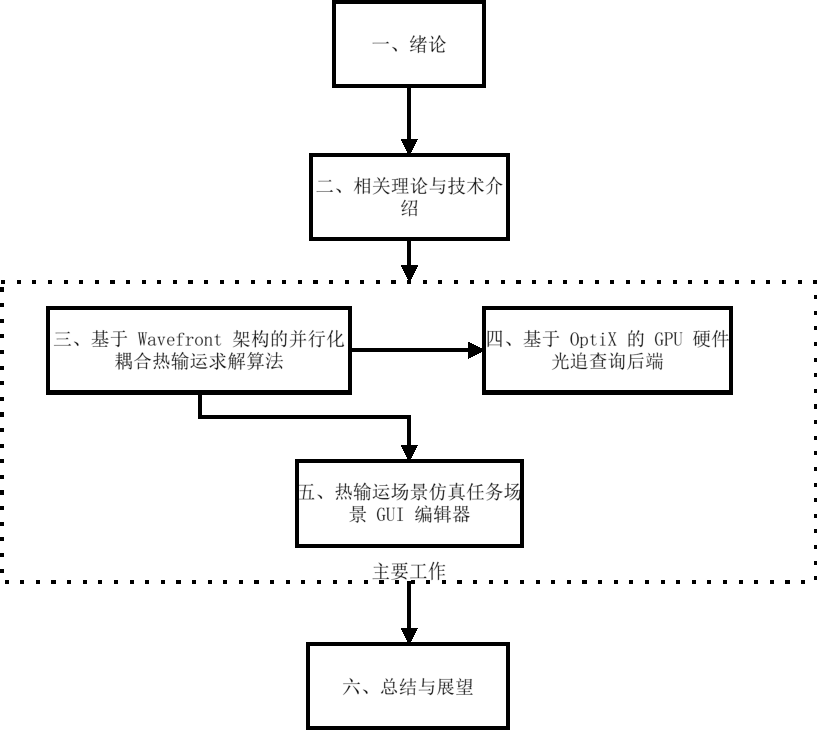
\includegraphics[width=0.95\textwidth]{Figures/ThesisArch/ThesisArch.pdf}
  \bicaption{论文整体组织架构图}{Overall Organization Structure of the Thesis}
  \label{fig:thesis-structure}
\end{figure}

